\documentclass[12pt]{report}
\usepackage{commands}

\begin{document}

\large
\begin{center}
AMSC 660 Homework 6\\
Due Oct 11\\
By Marvyn Bailly\\
\end{center}
\normalsize
\hrule

%Good luck my man
%---------------%
%---Problem 1---%
%---------------%


\begin{problem}%[vskip]
\subsection*{Problem 1}

Do \textbf{matrix completion} in two ways
\begin{enumerate}
    \item [(a)]
    Use the low-rank factorization model $A \approx XY^\top$ and the objective function of the form
    \[
         F(X,Y) = \frac{1}{2}\norm{P_\Omega(A - XY^\top)}_F^2 + \frac{\lambda}{2}(\|X\|_N^2 + \|Y\|_N^2).
    \]
    Try values of $\lambda = 0.1, 1, \and 10$, and $\text{rank}(X) = \text{rank}(Y) = k$, $k=1,2,\dots,7$. Find $X$ and $Y$ using alternating iteration
    \begin{align*}
        X^{m+1} &= \arg \min_X F(X,Y^m),\\
        Y^{m+1} &= \arg \min_Y F(X^{m+1},Y^m).
    \end{align*}
    Each of these steps can be further decomposed into a collection of small linear least squares problems. For example, at each substep of (1), we solve the linear least squares problem to compute the row $i$ of $X$:
    \[
        \mathbf{x}_i^\top = \arg \min_\mathbf{x}\frac{1}{2}\norm{\mathbf{x}^\top Y_{\Omega_i} - a_{\Omega_i}}_2^2 + \frac{\lambda}{2}\|x\|^2,
    \]
    where $\Omega_i := \brac{j | (i,j) \in \Omega}$. A similar problem can be set up for each column of $Y$. Work out solutions to these problems in a manner similar to the one in Sections 5.3.1 and 5.3.2 of LinearAlgebra.pdf except that there will be no constraint requiring the entries to be positive. Implement the resulting algorithm. Comment on how the value of $\lambda$ and the choice of rank affects the result. Which values of the rank and $\lambda$ seem the most reasonable to you? You can judge by your own row.

    \item [(b)] Use the approach of penalizing the nuclear norm in Section 6.3 of LinearAlgebra.pdf and the iteration
    \[
         M^{j+1} = S_\lambda (M^j + P_\Omega(A - M^j)).
    \]
    Experiment with different values of $\lambda$.  
\end{enumerate} 
Compare these two approaches for matrix completion. Which one gives more sensible
results? Which one is easier to use? Which one do you find more efficient?



\subsection*{Solution}
\begin{proof}

We wish to use the low-rank factorization model $A \approx XY^\top$ and the objective function of the form
\[
    F(X,Y) = \frac{1}{2}\norm{P_\Omega(A - XY^\top)}_F^2 + \frac{\lambda}{2}(\|X\|_N^2 + \|Y\|_N^2).
\]
We will find $X$ and $Y$ using alternating iterations of the form
\begin{align}
    X^{m+1} &= \arg \min_X F(X,Y^m),\\
    Y^{m+1} &= \arg \min_Y F(X^{m+1},Y^m).
\end{align}
We will compute the update of $X$ given by Eq. (1) by solving a smaller least squares problem for each row $i$ of $X$ of the form
\[
    \mathbf{x}_i^\top = \arg \min_\mathbf{x}\frac{1}{2}\norm{\mathbf{x}^\top Y_{\Omega_i} - a_{\Omega_i}}_2^2 + \frac{\lambda}{2}\|x\|^2.
\]
To solve the least squares problem, fix $Y$ and let $H = Y_{\Omega_i}$ and $b^\top = a_{\Omega_i}$. Observe that
\begin{align*}
    \frac{1}{2}\norm{x^\top H - b^\top}_2^2 + \frac{\lambda}{2}\norm{x}_2^2 &= \frac{1}{2}\norm{H^\top x - b}_2^2 + \frac{\lambda}{2}\norm{x}_2^2\\
    &= \frac{1}{2}\abrac{H^\top x - b,H^\top x - b} + \frac{\lambda}{2}\abrac{x,x}\\
    &= \frac{1}{2}(H^\top x - b)^\top(H^\top x - b) + \frac{\lambda}{2}x^\top x\\
    &= \frac{1}{2}(x^\top H - b^\top)(H^\top x - b) + \frac{\lambda}{2}x^\top x\\
    &= \frac{1}{2}x^\top H H^\top x - \frac{1}{2}b^\top H^\top x - \frac{1}{2}x^\top H b - \frac{1}{2}b^\top b + \frac{\lambda}{2}x^\top x\\
    &= \frac{1}{2}x^\top\paren{HH^\top + \lambda I}x - b^\top H x + \frac{1}{2}b^\top b =: \phi(x).\\
\end{align*} 
Now we wish to minimize the quadratic function $\phi(x)$. Noticing that $(HH^\top + \lambda I)$ is SPD, we can take the gradient and get
\[
    \nabla \phi(x) = \paren{HH^\top + \lambda I}x - Hb = 0,
\]
which means that the minimizer of $\phi(x)$ is given by
\begin{equation} \label{xupdate}
    x^* = (HH^\top + \lambda I)^{-1} Hb.
\end{equation}
Similarly, we will solve the update to the columns of $Y$ given by Eq. (2) by solving a smaller least squares problem for each row $j$ of $Y$ of the form
\[
    \mathbf{y}_j = \arg \min_\mathbf{y}\frac{1}{2}\norm{X_{\Omega_j}\mathbf{y}  - a_{\Omega_j}}_2^2 + \frac{\lambda}{2}\|y\|^2.
\]
To solve the least squares problem, fix $X$ and let $W = X_{\Omega_j}$ and $b = a_{\Omega_j}$. Observe that
\begin{align*}
    \frac{1}{2}\norm{Wy - b}_2^2 + \frac{\lambda}{2}\norm{y}_2^2 &= \frac{1}{2}\abrac{Wy - b,Wy - b} + \frac{\lambda}{2}\abrac{y,y}\\
    &= \frac{1}{2}(Wy - b)^\top(Wy - b) + \frac{\lambda}{2}y^\top y\\
    &= \frac{1}{2}(y^\top W^\top - b^\top)(Wy - b) + \frac{\lambda}{2}y^\top y\\
    &= \frac{1}{2}y^\top W^\top Wy - \frac{1}{2}y^\top W^\top b - \frac{1}{2}b^\top Wy + \frac{1}{2}b^\top b + \frac{\lambda}{2}y^\top y\\
    &= \frac{1}{2}y^\top \paren{W^\top W + \lambda I}y - y^\top W^\top b + \frac{1}{2}b^\top b =: \psi(y)\\
\end{align*} 
Now we wish to minimize the quadratic function $\psi(y)$. Noticing that $(W^\top W + \lambda I)$ is SPD, we can take the gradient and get
\[
    \nabla \psi(y) = \paren{W^\top W + \lambda I}y - W^\top b = 0,
\]
which means that the minimizer of $\psi(y)$ is given by
\begin{equation} \label{yupdate}
    y^* = (W^\top W + \lambda I)^{-1} W^\top b.
\end{equation}
Now we will implement the alternating iteration of Eq.(1) by updating the rows via \fullref{xupdate} and Eq.(2) by updating the columns via \fullref{yupdate} in MatLab. We will test the values $\lambda = 0.1, 1, \and 10$ with $\text{rank}(X) = \text{rank}(Y) = k$ where $k=1,\dots,7$ and $X$ and $Y$ are initialized as random matrices with entries uniformly disturbed between 0 and 1. Prior to matrix completion, my row looked like
\begin{verbatim}
    My row before completion:[3,4,0,0,4,3,5,0,4,4,5,3,0,5,0,5,2,4,5,3]
\end{verbatim}
Note, that for the sake of presentation, I will be showing only the first $10$ entries and rounding to tenths. Now let's test the different $\lambda$ values. We know that $\lambda$ affects the amount of penalization on the approximation. So we suspect that lower $\lambda$ values will suppress noise less and have more outliers while larger $\lambda$ values will suppress noise and outliers. Trying $\lambda = 0.1$ for $k=3,5,7$ and printing the results yields
\begin{verbatim}
    the absolute value of results subtracted from original entries:
    lambda = 0.1 and k = 3:[0.2,0.6,6.1,3.3,0.1,0.2,0.6,4.9,0.5,0.2]
    lambda = 0.1 and k = 5:[0.2,0.6,6,2.7,0.2,0.1,0.5,4.9,0.6,0]
    lambda = 0.1 and k = 7:[0.3,0.6,4.5,3.4,0.1,0.1,0.4,4.9,0.9,0.3]
    lambda = 1 and k = 3:[0,0.5,4.3,3.5,0.3,0.3,0.7,4.9,0.4,0.2]
    lambda = 1 and k = 5:[0.2,0.5,4.5,3.5,0,0.1,1,4.9,0.4,0.2]
    lambda = 1 and k = 7:[0.1,0.7,4.7,3.4,0.1,0.1,0.8,4.9,0.4,0.1]
    lambda = 10 and k = 3:[0.7,0.1,3.7,3.8,0.5,0,1.2,4.2,0.3,0.4]
    lambda = 10 and k = 5:[0.7,0.1,3.7,3.8,0.5,0,1.2,4.2,0.3,0.4]
    lambda = 10 and k = 7:[0.7,0.1,3.7,3.8,0.5,0,1.2,4.2,0.4,0.4]

    result values:
    lambda = 10 and k = 3:[3.7,3.9,3.7,3.8,3.5,3,3.8,4.2,3.7,3.6]
    lambda = 10 and k = 5:[3.7,3.9,3.7,3.8,3.5,3,3.8,4.2,3.7,3.6]
    lambda = 10 and k = 7:[3.7,3.9,3.7,3.8,3.5,3,3.8,4.2,3.6,3.6] 
\end{verbatim}
We see that for $\lambda = 0.1$ we have outliers such as $6$ which makes no sense in this context since we want movie rantings that are between 0 and 5, so this $\lambda$ value is too small. On the other hand, $\lambda = 10$ changes my previous response at a higher than $\lambda = 1$ and makes all of the entries more uniform, so I think $\lambda = 1$ will work best. To find a good $k$ value, notice that $k$ controls the number of latent factors used to approximate. Too small or too large of a $k$ may under- or overfit the data. Printing the results
\begin{verbatim}
    the absolute value of results subtracted from original entries:
    lambda = 1 and k = 1:[0.9,0.1,4.2,4,0.3,0.3,0.9,4.5,0,0.2]
    lambda = 1 and k = 2:[0.2,0.2,4.7,3.3,0.1,0.5,0.6,4.4,0.3,0.2]
    lambda = 1 and k = 3:[0,0.5,4.3,3.5,0.3,0.3,0.7,4.9,0.4,0.2]
    lambda = 1 and k = 4:[0.2,0.5,4.8,3.5,0.2,0.1,0.7,4.8,0.4,0.3]
    lambda = 1 and k = 5:[0.2,0.5,4.5,3.5,0,0.1,1,4.9,0.4,0.2]
    lambda = 1 and k = 6:[0.2,0.4,4.5,3.5,0,0.1,0.9,4.9,0.5,0.2]
    lambda = 1 and k = 7:[0.1,0.7,4.7,3.4,0.1,0.1,0.8,4.9,0.4,0.1]
\end{verbatim}
we see that $k = 5$ or $k = 6$ do Similarly well at keeping true to my results. From what I've heard about the movies I haven't seen, these values also do a decent job of predicting my reviews. I also tried taking the SVD of the original data matrix and looked at the number of most significant singular values which was also around $6$ singular values which corresponds to my findings but I'm not sure if there is a correlation. The algorithm was implemented into MatLab as follows:
\begin{python}
    function [X,Yt] = lowRankFact(A, l,k,nanLocations)
        [n,d] = size(A);
        X = ones(n,k);
        Yt = ones(k,d);
        for m = 1:100
            for i = 1:n
                YOmega = Yt;
                YOmega(:,nanLocations(i,:)) = [];
                bt = A(i,:);
                bt(nanLocations(i,:)) = [];
                HHt = YOmega*YOmega';
                X(i,:) = (HHt + l*eye(size(HHt))) \ YOmega*bt';
            end
            for j = 1:d
                XOmega = X;
                XOmega(nanLocations(:,j),:) = [];
                bt = A(:,j);
                bt(nanLocations(:,j)) = [];
                WtW = XOmega'*XOmega; %'
                Yt(:,j) = (WtW+l*eye(size(WtW))) \ XOmega'*bt; %'
            end
        end
    end
\end{python}


\noindent
Next, we wish to use the nuclear norm method of the form
\[
    M^{j+1} = S_\lambda (M^j + P_\Omega(A - M^j)).
\]
Experimenting with different $\lambda$ values, we find that $\lambda$ has a similar effect on the rankings as prior. A lower $\lambda$ value will suppress noise less and have more outliers while larger $\lambda$ values will suppress noise and outliers. So we pick $\lambda$ values near 1 which seem to be a good value to preserve my original rankings
\begin{verbatim}
    lambda = 1:[3.1,4.1,3.9,3.4,4,3,4.8,4.3,4,3.9]
    lambda = 10:[3.5,3.9,3.8,3.7,3.5,2.9,3.8,4.2,3.7,3.6]
\end{verbatim}
I find these values very good at staying true to my original ratings while making a reasonable prediction for the unknown values. The algorithm implemented into MatLab is as follows
\begin{python}
    function M = nuclear(A,l,nanLocations)
    M = rand(size(A));
   for i=1:1000
        AM = A - M;
        AM(nanLocations) = 0;
        Pomega = AM;
        [U,S,V] = svd(M + Pomega,'econ'); %slightly faster computation times
        Slambda = max(S - ;*eye(size(S)), 0);
        M = U*Slambda*V';
    end
end
\end{python}

\noindent 
Comparing the two methods, the low-rank factorization model runs slightly slower than the nuclear suggesting that the nuclear trick is slightly more efficient than the low-rank. This can be seen using MatLab's \verb+tic+ and \verb+toc+ functions which show that the low-rank takes on average $0.10$ seconds longer than the nuclear norm to complete $1000$ iterations. I enjoyed the amount of freedom the low-rank factorization method allowed by adjusting the two variables. On the other hand, it was easier and faster to fund appropriate $\lambda$ values that matched my movie ratings for the nuclear norm method. In summary, I think the low-rank method, allows more freedom to adjust the parameters but is slightly more inefficient. The nuclear norm method is more efficient at the cost of freedom in the parameters but is also easier to use. 

\noindent
All code can be found at: \url{https://github.com/MarvynBailly/AMSC660/tree/main/homework6}



\end{proof}
\end{problem}




%---------------%
%---Problem 2---%
%---------------%


\begin{problem}%[vskip]
\subsection*{Problem 2}

Extract a complete submatrix from the dataset MovieRankingData.csv by visual inspection with as many columns as you can find. This reduced dataset is needed for practicing algorithms for nonnegative matrix factorization (NMF).

\noindent
Compute the NMF $A \approx WH$ where $W$ has $k$ columns using
\begin{enumerate}
    \item [(a)] Projected gradient descend.
    \item [(b)] Lee-Seung scheme.
\end{enumerate}
Plot the Frobenius norm squared vs. iteration number for each solver. Which one do you find to be the most efficient?


\subsection*{Solution}
\begin{proof}

We begin by finding a submatrix of the dataset via visual inspection that has as many columns as we can find. We wish to compute the NMF $A \approx WH$ where $W$ has $k$ columns using Projected gradient descent and the Lee-Seung scheme. We will use a \verb+tol=10e-12+ to terminate the algorithms.

\noindent
We implemented the Projected gradient descend method using the following algorithm in MatLab:
\begin{python}
function errs = PJD(A,k,tol)
    a = 1/100;
    [n,d] = size(A);
    W = rand(n,k);
    H = rand(k,d);
    R = A - W*H;
    errs = [norm(R,'fro')]
    while tol < norm(R)
        W = max(W + a*R*H',0);
        R = A - W*H;
        H = max(H + a*W'*R,0);
        R = A - W*H;
        errs = [errs, norm(R,'fro')];
    end
end
\end{python}
Experimenting with different step sizes we found $a=1/100$ to be an appropriate value as when the step size was too small, the function would not converge.

\noindent
We implemented the Lee-Seung scheme using the following algorithm in MatLab:
\begin{python}
function errs = leeseung(A,k,tol)
    [n,d] = size(A);
    
    W = rand(n,k);
    H = rand(k,d);
    R = A - W*H;
    errs = [norm(R,'fro')]

    while tol < norm(R)
        W = (W .* (A*H')) ./ (W*(H*H'));
        H = (H .* (W'*A)) ./ ((W'*W)*H);
        R = A - W*H;
        errs = [errs, norm(R,'fro')];
    end
end
\end{python}

Plotting the Frobenius norm squared of the residual for each iteration number of the respective plots, we found the Lee-Seung scheme to be consistently more efficient across different $k$ values and different step sizes for Projected Gradient Descend as seen in Figures 1-4.

\noindent All code can be found at: \url{https://github.com/MarvynBailly/AMSC660/tree/main/homework6}

\begin{figure}[H]
    \begin{subfigure}[b]{0.5\linewidth}
        \centering
        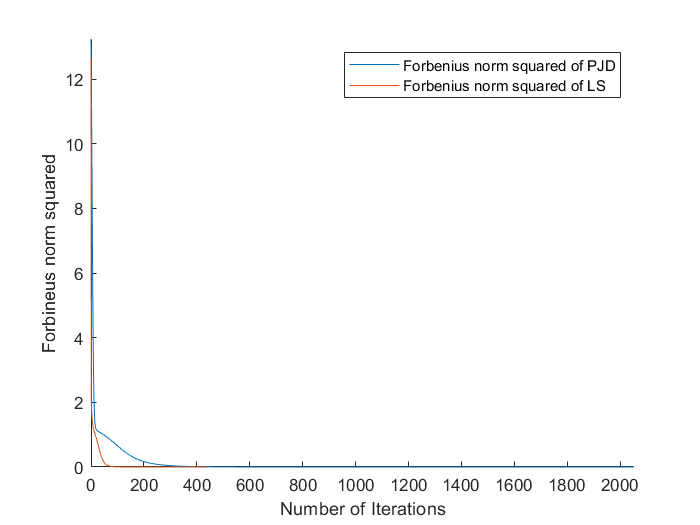
\includegraphics[width=\linewidth]{images/k3l.png}
        \caption{Zoomed out to see all Projected Gradient Descend iterations.}
        \label{fig1:a}
        \vspace{4ex}
    \end{subfigure}%%
    \begin{subfigure}[b]{0.5\linewidth}
        \centering
        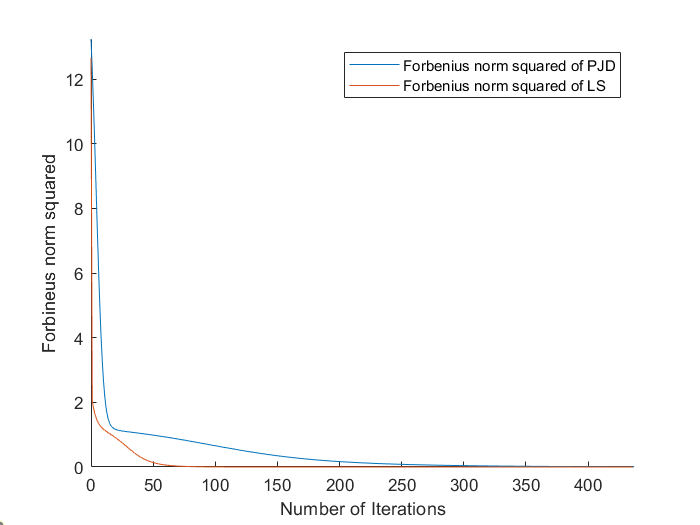
\includegraphics[width=\linewidth]{images/k3s.png}
        \caption{Zoomed in to see all Lee-Seung iterations.}
        \label{fig1:b}
        \vspace{4ex}
    \end{subfigure}
    \caption{Frobenius norm squared of each iteration of Projected Gradient Descend (seen in blue) and Lee-Seung (seen in orange) for $k=3$ and Projected Gradient Descent with step size of $a=1/100$}
    \label{fig1}
\end{figure}

\begin{figure}[H]
    \begin{subfigure}[b]{0.5\linewidth}
        \centering
        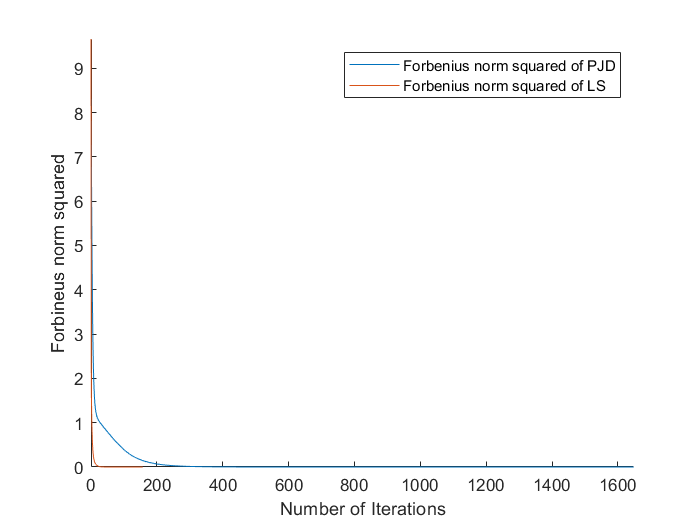
\includegraphics[width=\linewidth]{images/k7l.png}
        \caption{Zoomed out to see all Projected Gradient Descend iterations.}
        \label{fig2:a}
        \vspace{4ex}
    \end{subfigure}%%
    \begin{subfigure}[b]{0.5\linewidth}
        \centering
        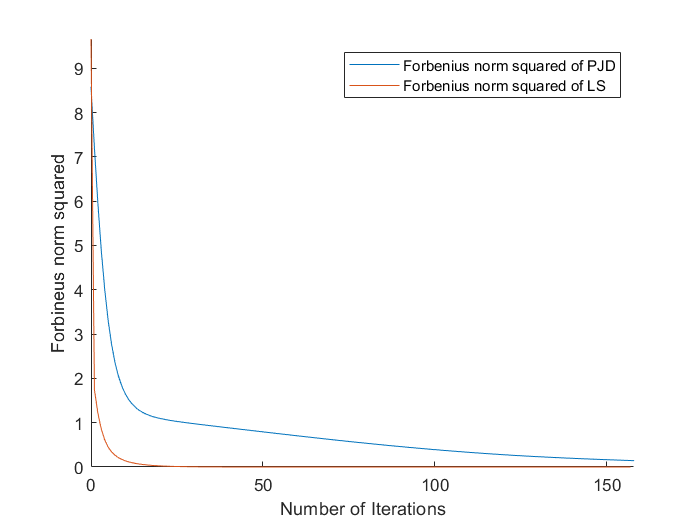
\includegraphics[width=\linewidth]{images/k7s.png}
        \caption{Zoomed in to see all Lee-Seung iterations.}
        \label{fig2:b}
        \vspace{4ex}
    \end{subfigure}
    \caption{Frobenius norm squared of each iteration of Projected Gradient Descend (seen in blue) and Lee-Seung (seen in orange) for $k=7$ and Projected Gradient Descent with step size of $a=1/100$}
    \label{fig2}
\end{figure}

\begin{figure}[H]
    \begin{subfigure}[b]{0.5\linewidth}
        \centering
        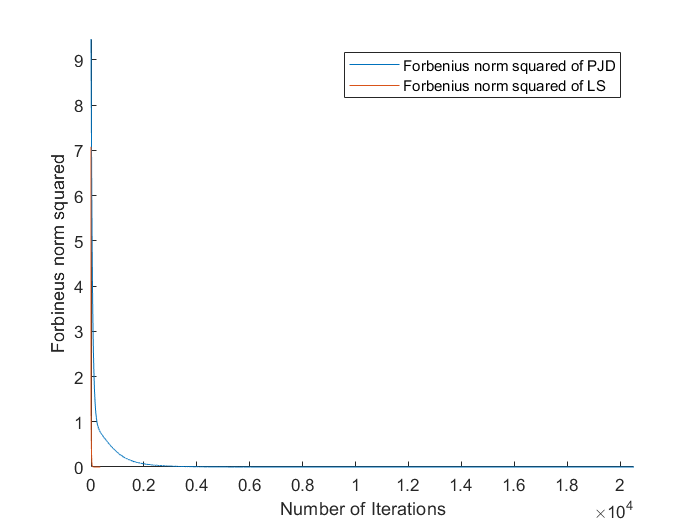
\includegraphics[width=\linewidth]{images/k7la1000.png}
        \caption{Zoomed out to see all Projected Gradient Descend iterations.}
        \label{fig3:a}
        \vspace{4ex}
    \end{subfigure}%%
    \begin{subfigure}[b]{0.5\linewidth}
        \centering
        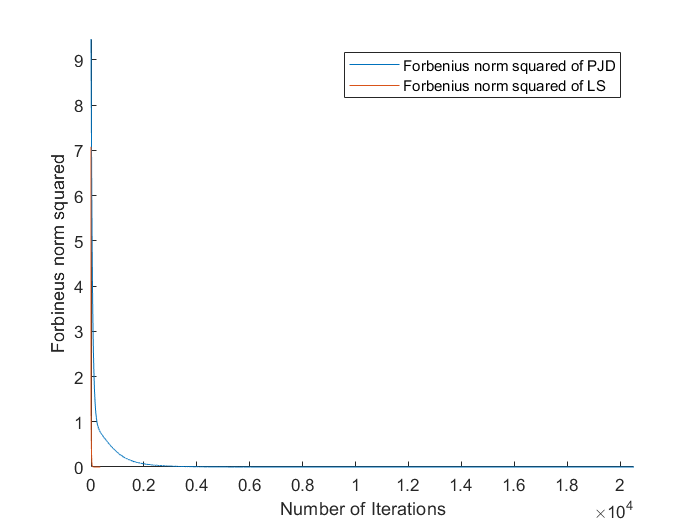
\includegraphics[width=\linewidth]{images/k7la1000.png}
        \caption{Zoomed in to see all Lee-Seung iterations.}
        \label{fig3:b}
        \vspace{4ex}
    \end{subfigure}
    \caption{Frobenius norm squared of each iteration of Projected Gradient Descend (seen in blue) and Lee-Seung (seen in orange) for $k=7$ and Projected Gradient Descent with stepsize of $a=1/1000$}
    \label{fig3}
\end{figure}

\begin{figure}[H]
    \begin{subfigure}[b]{0.5\linewidth}
        \centering
        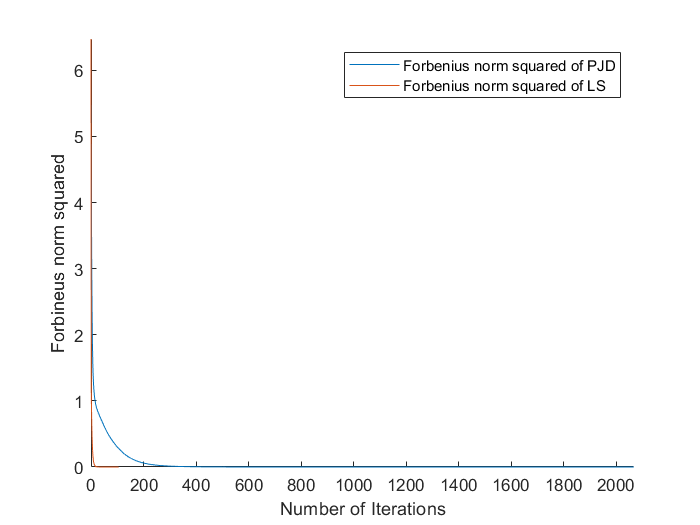
\includegraphics[width=\linewidth]{images/k10l.png}
        \caption{Zoomed out to see all Projected Gradient Descend iterations.}
        \label{fig4:a}
        \vspace{4ex}
    \end{subfigure}%%
    \begin{subfigure}[b]{0.5\linewidth}
        \centering
        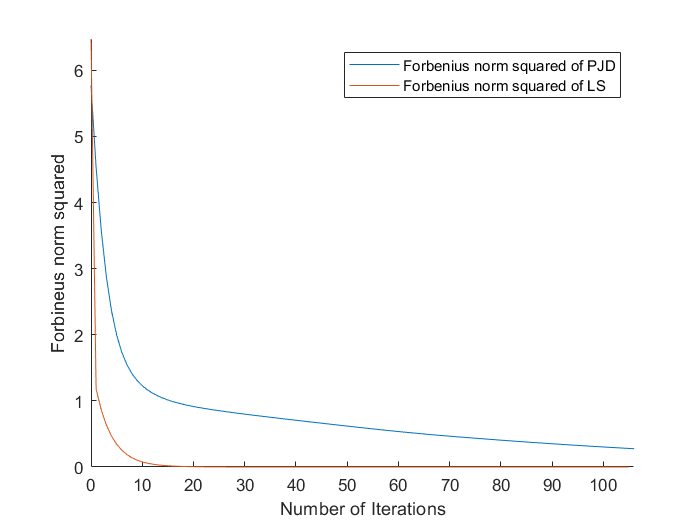
\includegraphics[width=\linewidth]{images/k10s.png}
        \caption{Zoomed in to see all Lee-Seung iterations.}
        \label{fig4:b}
        \vspace{4ex}
    \end{subfigure}
    \caption{Frobenius norm squared of each iteration of Projected Gradient Descend (seen in blue) and Lee-Seung (seen in orange) for $k=10$ and Projected Gradient Descent with stepsize of $a=1/100$}
    \label{fig4}
\end{figure}
\end{proof}
\end{problem}






\end{document}